
\paragraph{Khatri-Rao product}
The Khatri-Rao product is the column-wise Kronecker product~\citep{smilde2005multi,bro1998multi}. Let $\Ab\in\RR^{m\times R}$ and $\Bb\in\RR^{n\times R}$. The Khatri-Rao product of $\Ab$ and $\Bb$, denoted as $\Ab\krao\Bb\in\RR^{mn\times R}$, is defined by
\begin{align*}
    \def\baseline{-0.5ex}
    \Ab\krao\Bb =
    \begin{bmatrix}
    \vline & \vline  &   & \vline \\
    \ab_1\kron\bb_1 & \ab_2\kron\bb_2 & \dots & \ab_R\kron\bb_R\\
    \vline & \vline & & \vline 
    \end{bmatrix}
=
    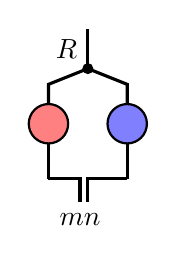
\begin{tikzpicture}[baseline=\baseline]
    \tikzset{tensor/.style = {minimum size = 0.5cm,shape = circle,thick,draw=black,inner sep = 0pt}, edge/.style   = {thick,line width=.4mm},every loop/.style={}}
    \def\y{0}
    \def\x{0}
    \node[tensor,fill=red!50!white] (A) at (\x,\y){$\Ab$};
    \node[tensor,fill=blue!50!white] (B) at (\x+1,\y){$\Bb$};
    \draw[edge] (\x,\y+0.25) -- (\x,\y+0.5) -- (\x+0.5,\y+0.7);
    \draw[edge] (\x+1,\y+0.25) -- (\x+1,\y+0.5) -- (\x+0.5,\y+0.7);
    \draw[edge] (\x+0.5,\y+0.7) -- (\x+0.5,\y+1.2) node [left, midway] {\edgelabel{$R$}};
    \draw  node[fill = black,circle,inner sep=0pt,minimum size=4pt] (m) at (\x+0.5,\y+0.7) {};
    \draw[edge] (\x,\y-0.25) -- (\x,\y-0.7);
    \draw[edge] (\x+1,\y-0.25) -- (\x+1,\y-0.7);
    \draw[edge] (\x+1,\y-0.7) -- (\x+0.5,\y-0.7) -- (\x+0.5,\y-1);
    \draw[edge] (\x+1,\y-0.25) -- (\x+1,\y-0.7);
    \draw[edge] (\x,\y-0.7) -- (\x+0.4,\y-0.7) -- (\x+0.4,\y-1)node [below] {\edgelabel{$mn$}};
    \end{tikzpicture}\hspace{0.5cm},
\end{align*}
where $\ab_1,\dots,\ab_R\in\RR^{m}$ are the columns of $\Ab$ and $\bb_1,\dots,\bb_R\in\RR^{n}$ are the columns of $\Bb$.  In the corresponding tensor network diagram, the copy tensor enforces that the resulting matrix only contains the Kronecker product of \emph{matching} columns of $\Ab$ and $\Bb$. 
\begin{remark}
Some of the Khatri-Rao product properties are listed below:
\begin{enumerate}
\item Like the Kronecker product, the Khatri-Rao product is not commutative, i.e., $\Ab\krao\Bb\neq \Bb\krao\Ab$ in general.
\item The Khatri-Rao product is associative, i.e., $\Ab\krao(\Bb\krao\Cb)=(\Ab\krao\Bb)\krao\Cb$, where $\Ab\in\RR^{m\times R},\Bb\in\RR^{n\times R}$ and $\Cb\in\RR^{s\times R}$.
\item The columns of $\Ab\krao\Bb$ form a subset of the columns of the Kronecker product $\Ab\kron \Bb$.
\end{enumerate}
\end{remark}

\paragraph{Hadamard product}
Let $\Ab\in\RR^{m\times n}$ and $\Bb\in\RR^{m\times n}$ be matrices of the same shape. The Hadamard (or component-wise) product of $\Ab$ and $\Bb$ is the matrix  $\Ab\hadam\Bb\in\RR^{m\times n}$ defined element-wise by 
$$(\Ab\hadam\Bb)_{ij} = \Ab_{ij}\Bb_{ij}.$$
In tensor network diagrams, the Hadamard product can easily be represented using copy tensors:
\begin{equation*}
\Ab\hadam\Bb =
     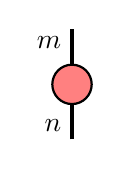
\begin{tikzpicture}[baseline=\baseline]
    \tikzset{tensor/.style = {minimum size = 0.5cm,shape = circle,thick,draw=black,inner sep = 0pt}, edge/.style   = {thick,line width=.4mm},every loop/.style={}}
    \def\y{0}
    \def\x{0}
    \draw[edge] (\x,\y-0.7) -- (\x,\y+0.7)  node [very near end,left] {\edgelabel{$m$}} node [very near start,left] {\edgelabel{$n$}} ;
    \node[tensor,fill=red!50!white] (A) at (\x,\y){$\Ab$};
    \end{tikzpicture} 
    \ \hadam %
    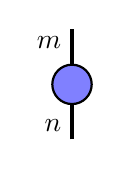
\begin{tikzpicture}[baseline=\baseline]
    \tikzset{tensor/.style = {minimum size = 0.5cm,shape = circle,thick,draw=black,inner sep = 0pt}, edge/.style   = {thick,line width=.4mm},every loop/.style={}}
    \def\y{0}
    \def\x{0}
    \draw[edge] (\x,\y-0.7) -- (\x,\y+0.7)node [very near end,left] {\edgelabel{$m$}} node [very near start,left] {\edgelabel{$n$}} ;
    \node[tensor,fill=blue!50!white] (B) at (\x,\y){$\Bb$};
    \end{tikzpicture}
\ =
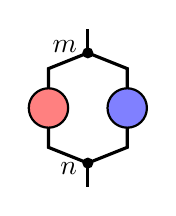
\begin{tikzpicture}[baseline=\baseline]
    \tikzset{tensor/.style = {minimum size = 0.5cm,shape = circle,thick,draw=black,inner sep = 0pt}, edge/.style   = {thick,line width=.4mm},every loop/.style={}}
    \def\y{0}
    \def\x{0}
    \node[tensor,fill=red!50!white] (A) at (\x,\y){$\Ab$};
    \node[tensor,fill=blue!50!white] (B) at (\x+1,\y){$\Bb$};
    \draw[edge] (\x,\y+0.25) -- (\x,\y+0.5) -- (\x+0.5,\y+0.7);
    \draw[edge] (\x+1,\y+0.25) -- (\x+1,\y+0.5) -- (\x+0.5,\y+0.7);
    \draw[edge] (\x+0.5,\y+0.7) -- (\x+0.5,\y+1) node [near start,left] {\edgelabel{$m$}};
    \draw  node[fill = black,circle,inner sep=0pt,minimum size=4pt] (m) at (\x+0.5,\y+0.7) {};
    \draw[edge] (\x,\y-0.25) -- (\x,\y-0.5) -- (\x+0.5,\y-0.7);
    \draw[edge] (\x+1,\y-0.25) -- (\x+1,\y-0.5) -- (\x+0.5,\y-0.7);
    \draw[edge] (\x+0.5,\y-0.7) -- (\x+0.5,\y-1) node [near start,left] {\edgelabel{$n$}};
    \draw  node[fill = black,circle,inner sep=0pt,minimum size=4pt] (m) at (\x+0.5,\y-0.7) {};
\end{tikzpicture}.
\end{equation*}
More generally, for any $\Ab_1\in\RR^{m\times n},\dots,\Ab_d\in\RR^{m\times n}$ we have 
\begin{align*}
\Ab_1\hadam\Ab_2\dots\hadam\Ab_{d} 
=
    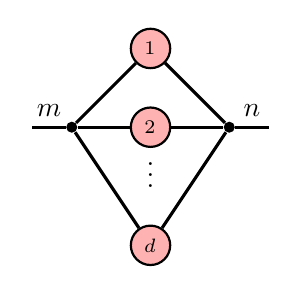
\begin{tikzpicture}[baseline=\baseline]
    \tikzset{tensor/.style = {minimum size = 0.5cm,shape = circle,thick,draw=black,inner sep = 0pt}, edge/.style   = {thick,line width=.4mm},every loop/.style={}}
    \def\y{1}
    \def\x{0}
    \node[tensor,fill=red!30!white] (A_1) at (\x,\y){$\Ab_1$};
    \node[tensor,fill=red!30!white] (A_2) at (\x,\y-1){$\Ab_2$};
    \node[draw=none] at (\x,\y-1.5) {\scalebox{1}{\textcolor{black}{$\vdots$}}};
    \node[tensor,fill=red!30!white] (A_N) at (\x,\y-2.5){$\Ab_d$};
    \draw  node[fill = black,circle,inner sep=0pt,minimum size=4pt] (m) at (\x+1,\y-1) {};
    \draw  node[fill = black,circle,inner sep=0pt,minimum size=4pt] (n) at (\x-1,\y-1) {};
    \draw[edge] (A_1) -- (m);
    \draw[edge] (A_2) -- (m);
    \draw[edge] (A_N) -- (m);
    \draw[edge] (A_1) -- (n);
    \draw[edge] (A_2) -- (n);
    \draw[edge] (A_N) -- (n);
    \draw[edge] (m) -- (\x+1.5,\y-1)node [midway,above] {\edgelabel{$n$}};
    \draw[edge] (n) -- (\x-1.5,\y-1)node [midway,above] {\edgelabel{$m$}};
    \end{tikzpicture}.
\end{align*}
\begin{remark}
We list here some useful properties of the Hadamard product.
\begin{itemize}
    \item The Hadamard product of a tensor $\Tt$ with entries in $\{0,1\}$ with itself is $\Tt$. This is in particular true for the copy tensor:
    
    Let $\Tt\in\RR^{d_1\times d_2\times d_3}$ be a 3rd way copy tensor. Then the Hadamard product $\Tt\hadam\Tt$ in tensor networks is:
    $$\Tt\hadam\Tt=
    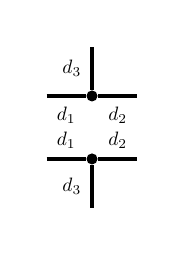
\begin{tikzpicture}[baseline=\baseline]
   \tikzset{tensor/.style = {minimum size = 0.5cm,shape = circle,thick,draw=black,inner sep = 0pt}, edge/.style = {thick,line width=.4mm},every loop/.style={}}
    \def\y{0.2}
    \def\x{0}
     \draw  node[fill = black,circle,inner sep=0pt,minimum size=4pt] (m) at (\x,\y-0.5) {};
     \draw  node[draw=none] (a) at (\x-0.7,\y-0.5) {};
     \draw  node[draw=none] (b) at (\x+0.7,\y-0.5) {};
     \draw  node[draw=none] (c) at (\x,\y-1.25) {};
    \draw[edge] (a) -- (m) node [midway,above] {\scalebox{0.7}{\dimcolor{$d_1$}}};
    \draw[edge] (m) -- (b)node [midway,above] {\scalebox{0.7}{\dimcolor{$d_2$}}};
    \draw[edge] (m) -- (c)node [midway,left] {\scalebox{0.7}{\dimcolor{$d_3$}}};
    \draw  node[fill = black,circle,inner sep=0pt,minimum size=4pt] (m1) at (\x,\y+0.3) {};
     \draw  node[draw=none] (d) at (\x-0.7,\y+0.3) {};
     \draw  node[draw=none] (e) at (\x+0.7,\y+0.3) {};
     \draw  node[draw=none] (f) at (\x,\y+1.05) {};
    \draw[edge] (d) -- (m1)node [midway,below] {\scalebox{0.7}{\dimcolor{$d_1$}}};
    \draw[edge] (m1) -- (e)node [midway,below] {\scalebox{0.7}{\dimcolor{$d_2$}}};
    \draw[edge] (m1) -- (f)node [midway,left] {\scalebox{0.7}{\dimcolor{$d_3$}}};
    \node[draw=none] at (\x,\y-0.15){$\hadam$};
\end{tikzpicture}
=
    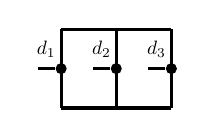
\begin{tikzpicture}[baseline=\baseline]
   \tikzset{tensor/.style = {minimum size = 0.5cm,shape = circle,thick,draw=black,inner sep = 0pt}, edge/.style = {thick,line width=.4mm},every loop/.style={}}
    \def\y{0}
    \def\x{0}
    \draw[edge](\x-0.7,\y-0.5)--(\x+0.7,\y-0.5);
    \draw[edge](\x-0.7,\y+0.5)--(\x+0.7,\y+0.5);
    \draw[edge](\x-0.7,\y-0.5)--(\x-0.7,\y+0.5);
    \draw[edge](\x+0.7,\y-0.5)--(\x+0.7,\y+0.5);
    \draw[edge](\x,\y+0.5) -- (\x,\y-0.5);
     \draw  node[fill = black,circle,inner sep=0pt,minimum size=4pt] (m1) at (\x-0.7,\y) {};
    \draw  node[fill = black,circle,inner sep=0pt,minimum size=4pt] (m) at (\x,\y) {};
    \draw  node[fill = black,circle,inner sep=0pt,minimum size=4pt] (m2) at (\x+0.7,\y) {};
    \draw[edge](m1)--(\x-1,\y)node [midway,above] {\scalebox{0.7}{\dimcolor{$d_1$}}};
    \draw[edge](m2)--(\x+0.4,\y)node [midway,above] {\scalebox{0.7}{\dimcolor{$d_3$}}};
    \draw[edge](m)--(\x-0.3,\y)node [midway,above] {\scalebox{0.7}{\dimcolor{$d_2$}}};
     \end{tikzpicture}$$
    
